%%%%%%%%%%%%%%%%%%%%%%%%%%%%%%%%%%%%%%%%%%%%%%%%%%%%%%%%%%%%%%%%%%%%%%%%%%%%%%%%%%%%%%%%%%%%%%%%%%%%%%
%
%   Filename    : appendix_D.tex
%
%   Description : This file will contain information about your Resource Persons
%                 
%%%%%%%%%%%%%%%%%%%%%%%%%%%%%%%%%%%%%%%%%%%%%%%%%%%%%%%%%%%%%%%%%%%%%%%%%%%%%%%%%%%%%%%%%%%%%%%%%%%%%%

\chapter{Preliminary Results}
\label{sec:appendixe}


In this section, an implementation of feature fusion, using the collected traffic and weather dataset, will be discussed through a feedforward ANN. To evaluate the performance of feature fusion, two experiments will be performed: predicting the traffic condition using weather variables only and predicting the traffic condition by applying feature fusion to both the traffic condition and weather variables.

\section{Data Pre-processing}
Before feeding the data to the ANN model, the data must be cleaned and processed. Recall that the collected dataset for both the weather and traffic are sampled at a 15-minute interval and an hourly interval respectively and that the traffic dataset contains missing records (see Section \ref{rd_datacollection}). Given these anomalies, interpolation must be done for the traffic dataset to supply the missing records and intervals, whereas resampling and interpolation must be performed for the weather dataset to match the traffic dataset’s interval.

\subsection{Traffic Dataset}
For the traffic dataset, we must first separate the records based on their respective road segments. For instance, we must have a separate dataset only containing the records from Taft Avenue, Quirino, Buendia and the other road segments. This is to ensure that our interpolation later on will not be influenced by other road segments rather than itself.

Before cleaning the data, we must consider that interpolation requires numerical values so that the missing values can be estimated. Therefore, we must convert the traffic conditions for both the northbound and southbound to their numerical equivalents. Since they are classified as light, moderate and heavy, we could rank them based on their intensities. As a result, light, moderate and heavy are classified into 0.0, 0.5 and 1.0 respectively. These values are chosen so that the min-max scaling normalization is no longer needed to perform later on.

Next, to clean the traffic dataset, we have to consider the two cases of missing data that it has: having \textit{none}(N) conditions and having a particular interval not recorded at all. To resolve the first case, first, we must remove all \textit{none}(N) condition from both the northbound and southbound traffic condition features. Next, we perform linear interpolation to fill in these filtered records. For the second case, we must fill in the unrecorded intervals. Hence, although the traffic dataset is already in our target series interval, we need to resample the dataset at a 15-minute interval so that all the intervals, including the missing ones, will be added. Next, we perform linear interpolation again to fill in these missing records.



\subsection{Weather Dataset}
Before processing our dataset, recall that our weather dataset contains 20 weather variables, having the temperature, heat index, dew point, wind chill and feels like on both their Celcius and Fahrenheit form, and wind speed and wind gust on both their miles per hour and kilometers per hour form. In our case, we opted to use their Celcius form and kilometers per hour form. Thus, scoping down our weather variables to 13.

For the weather dataset, since, fortunately, our data is complete per interval, we could directly start resampling our records. But, before this, we must ensure that our weather variables are in their numerical equivalents as a preparation for interpolation later on. In the case of our dataset, only the weather condition is in its categorical form. To rank the weather condition, we adapted \shortciteA{doi:10.1080/01998590309509243} approach of ranking weather conditions based on its attenuation of incoming solar radiation. With that, the weather condition data is ready for interpolation and is already normalized.

After processing our dataset, we could now match our weather dataset to the intervals of our traffic dataset. To do this, we must first resample our dataset at a 15-minute interval. Next, we perform linear interpolation to fill in the missing intervals, similar to how we filled the missing records from our traffic data.

\section{Input Dataset}
To scale down our experiment, we sampled three consecutive months of 2015 as our dataset (from September 2015 to November 2015) for both traffic and weather. Furthermore, we only used the traffic records of Taft Avenue with the weather of Manila as our input dataset. For the features, we only considered the southbound traffic condition for the traffic. On the other hand, we considered 13 features for the weather. These include temperature (in Celsius), wind speed (in kilometers per hour), weather condition, precipitation (in millimeters), humidity, visibility, pressure, cloud cover, heat index (in Celsius), dew point (in Celsius), wind chill (in Celsius), wind gust (in kilometers per hour), and feels-like (in Celsius). It must be noted, however, that the correlation of these features has not been considered in this experiment.


\section{Developing the Model}
Developing our feedforward ANN consists of 5 steps: preparing the data, defining the training and test data, building the ANN model itself, training the model and finally evaluating the model. Our model will be implemented using Python, utilizing the Keras library with Tensorflow. For our experiment, we would be performing two cases: predicting the traffic condition using weather variables only and predicting the traffic condition by applying feature fusion to both the traffic condition and weather variables.

\subsection{Preparing the Data}
Aside from the pre-processing that was performed earlier, we also have to perform some additional pre-processing targeted for our model. First, we have to merge both our traffic dataset and weather dataset. Since they already have matching intervals and the traffic dataset is already separated based on its road segments, we could simply merge it without any additional processing involved. It is important to note that only one road segment dataset will only be used per model, especially in our case where the weather dataset is the generalized weather for all road segments, since the generalized weather may be biased on a particular road segment.



Next, we remove the unnecessary features from our merged dataset. These include the road, road segment and the date and time, leaving us with the numerical traffic features and weather variable features. Finally, we must perform normalization to standardize the values. In our case, we performed min-max scaling normalization to scale our data from 0.0 to 1.0.



\subsection{Defining the Training and Testing Dataset}
The dataset is split into two sub-datasets: the training dataset which includes September 2015 to October 2015 and the testing dataset which includes November 2015. From this, the target label, the feature that we want to predict, and the training features, the features from which the prediction will be based on, are defined. To further minimize the scope of the experiment, we would only predict the traffic condition of the southbound lane. Thus, for the experiment, our target label would be the traffic condition of the southbound lane.

In order to illustrate the benefits of feature fusion, two experiments will be performed. First, the training features will be solely based on weather variable features. Second, the training features will include the traffic condition from the southbound lane and the weather variable features thus, performing feature fusion on the traffic and weather variables features. To further illustrate these experiments, Figures \ref{figure:prelim_exp1} and \ref{figure:prelim_exp2} show the diagram of these scenarios.




\begin{figure}[h]
\caption{Predict Southbound Traffic without Feature Fusion}
\centering
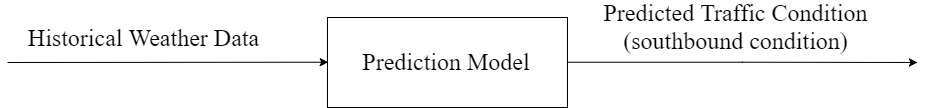
\includegraphics[width=0.8\textwidth]{prelim_exp1}
\label{figure:prelim_exp1}
\end{figure}

\begin{figure}[h]
\caption{Predict Southbound Traffic with Feature Fusion}
\centering
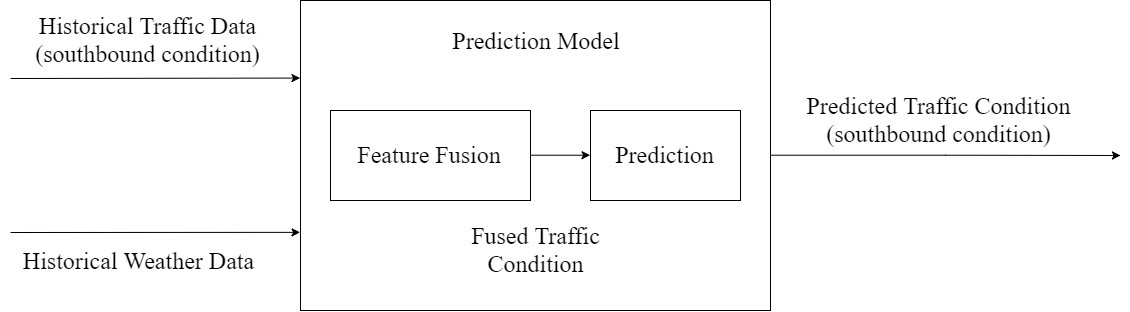
\includegraphics[width=0.8\textwidth]{prelim_exp2}
\label{figure:prelim_exp2}
\end{figure}

\subsection{Building the Model}
In building our feedforward ANN model, we used three densely-connected neural network layer: one for the input, one for the hidden layer and one for the output. For each of our experiments, both uses rectified linear unit (ReLU) as the activation function, and each has 13 input dimensions and 14 input dimensions respectively. The dimensions correspond to the number of training features that we will use for the model. The model has 13 weather variable features for our first experiment scenario, whereas we have 13 weather variable features and 1 traffic feature for our second scenario. For both experiments, it uses one hidden layer that similarly uses ReLU as its activation function, and has 8 input dimensions. It also has one output layer with only one output dimension for our southbound traffic condition. Figure \ref{prelim_model1} and \ref{prelim_model2} illustrate the diagram of these models.


\begin{figure}[h]
\caption{ANN Model for Predicting Southbound Traffic without Feature Fusion}
\centering
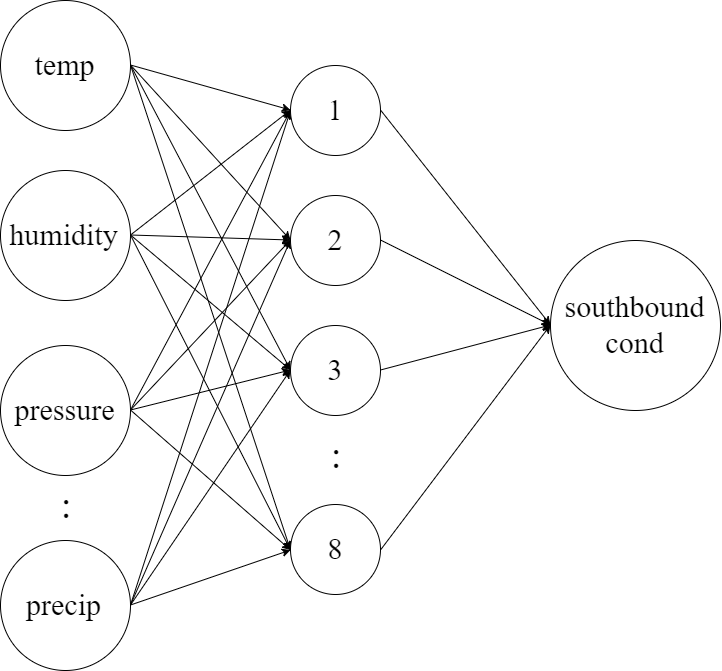
\includegraphics[width=0.5\textwidth]{prelim_model1}
\label{prelim_model1}
\end{figure}

\begin{figure}[h]
\caption{ANN Model for Predicting Southbound Traffic with Feature Fusion}
\centering
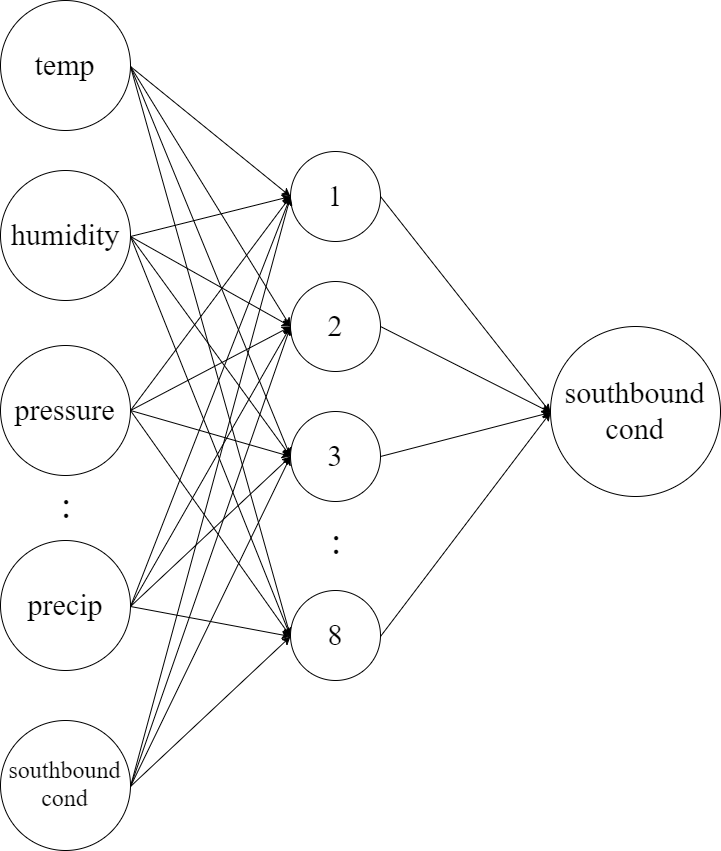
\includegraphics[width=0.5\textwidth]{prelim_model2}
\label{prelim_model2}
\end{figure}


\subsection{Training the Model}
In preparation for training the model, we configured the model’s optimizer, loss function, and evaluation metrics. For its optimizer, we set it to use the Adam optimizer, having a learning rate of 0.001 and a decay factor of 0.0. Meanwhile, for its loss function, we used mean squared error (MSE). Finally, for its evaluation metrics, we used mean absolute percentage error (MAPE). Using the training dataset, for both experiments, we trained the model using 1000 epochs and a batch size of 5. 



\subsection{Evaluation of the Model}
For the first experiment, where the model only uses weather variable features as its training features, the model generated a root-mean-square error (RMSE) of 6.57\% and a MAPE of 57,787,420\%. On the other hand, the second experiment, where the model uses feature fusion for the southbound traffic condition and weather variables as its training features, generated an RMSE of 0.0001\% and a MAPE of 8,396\%. Although the MAPE is quite high due to the lack of epochs, we could observe how massive the difference is between the first model and the second model. Given that, we can conclude that using feature fusion can significantly increase the accuracy of the model.
